\chapter{光分析法}

\section{光分析法导论}

\subsection{吸收、发射、荧光光谱}

\subsubsection{吸收光谱法}

物质吸收了辐射能,使辐射能的强度降低,这样的光谱被称为吸收光谱。

吸收光谱要求的物质状态:液态、固态、均质固态

\subsubsection{发射光谱法}

以火焰、电弧、等离子炬等作为能量源,使气态源自的外层电子受激发射出特征光谱进行
定性定量分析的方法。

\subsubsection{荧光光谱法}

也称为光致光谱,其光源为辐射能,物质受外界光能作用被激发,退激发的时候以辐射的
形式表现出来,即为荧光光谱。


\subsection{原子光谱和分子光谱}

原子光谱为分立的线状光谱,价电子能级跃迁。分子光谱为连续的带状光谱,分子能级跃
迁。

\section{紫外可见吸收光谱}

\subsection{紫外可见吸收光谱法及其原理}

\subsubsection{电子跃迁与分子吸收光谱}

\paragraph{电子能级} 此类吸收能量差 $\Delta E$ 较大 $1 \sim 2 \mathrm{eV}$。电
子跃迁产生的吸收光谱在紫外 $-$ 可见光区,称为紫外 $-$ 可见光谱或分子的电子光谱。

\paragraph{振动能级} 一般能量差 $\Delta E$ 约为 $ 0.05 \sim 1 \mathrm{eV}$,跃
迁产生的吸收光谱位于红外区,使用红外光谱或分子转动光谱。

\paragraph{转动能级} $\Delta E$ 为 $0.005 \sim 0.050 \mathrm{eV}$,跃迁产生吸收
光谱位于远红外区,使用远红外光谱或分子转动光谱。

\subsubsection{用途}

\begin{enumerate}
    \item 吸收光谱的波长分布是由产生谱带的跃迁能级间的能量差所决定,反映了分子
          内部能级的分布状况,是物质定性分析的依据。
    \item 吸收谱带的强度与分子偶极矩的变化,跃迁几率油光,也提供分子结构信息,
          将在最大吸收波长处测得的摩尔吸光系数 $\epsilon_{\max}$ 也作为定性分析的
          依据。
    \item 吸收谱带强度与该分子吸收的光子数成正比,可以作为定量分析的依据。
\end{enumerate}

紫外可见吸收光谱一般通过分子价电子能级跃迁产生,为连续的带状光谱。光谱的波长范
围一般是 $10 - 800 \ \mathrm{nm}$。测量透过率 $T$ 和吸收系数 $A$,可用于结构鉴
定和定量分析(既可以定性又可以定量)。

透过率 Transmittance $T$

\begin{equation}
    T = \frac{I_t}{I_0} \quad 0 \leq T \le 1
\end{equation}

吸光度 Absorbance $A$

\begin{equation}
    A = - \lg T
\end{equation}

\subsection{有机物电子跃迁与分子吸收光谱}

有机化合物的紫外 $-$ 可见吸收光谱是三种电子跃迁的结果:

$\sigma, \pi, n$ 电子跃迁。

当外层电子吸收紫外光或可见光辐射后,就从基态向激发态(反键轨道)跃迁。主要有四
种跃迁,所需的能量 $\Delta E$ 大小顺序为:

\begin{equation}
    \sigma \rightarrow \sigma^* > n \rightarrow \sigma^*
    > \pi \rightarrow \pi^* > n \rightarrow \pi^*
\end{equation}

\begin{figure}[H]
    \centering
    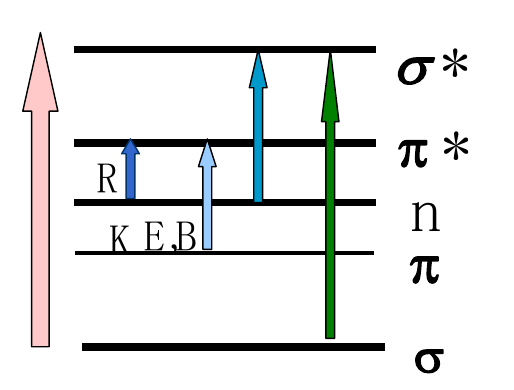
\includegraphics[width=0.35\textwidth]{images/UV-Vis-orbit.png}
    \caption{四种跃迁示意图}
\end{figure}


\subsubsection{$\sigma \rightarrow \sigma^*$ 跃迁}

此类跃迁所需能量最大,$\sigma$ 电子只有吸收远紫外光的能量才能发生跃迁,吸收波长
$\lambda < 200 nm$。饱和烷烃的分子吸收光谱出现在远紫外区,例如,$\ce{CH4}$ 的
$\lambda_{\max} = 125 \mathrm{nm}$,$\ce{CH3CH3}$ $\lambda_{\max} = 135
    \mathrm{nm}$。只能被真空紫外分光光度计检测到,作为溶剂使用。

\subsubsection{$n \rightarrow \sigma^*$ 跃迁}

吸收波长为 $ 150 \sim 250 \mathrm{nm} $,大部分在远紫外区,近紫外区仍不易观察到,
所需的能量较大。

含非键电子的饱和烃衍生物(含 $\ce{N}$、$\ce{O}$、$\ce{S}$和卤素等杂原子均呈现
$n \rightarrow \sigma^*$ 跃迁。

末端吸收:

醇类末端吸收不大,可以用作溶剂。

\begin{table}[H]
    \centering
    \caption{各化合物对应的 $\lambda_{\max}$ 和 $\epsilon_{\max}$}
    \begin{tabular}{ccc}
        \toprule
        化合物           & $\lambda_{\max} (\mathrm{nm})$ & $ \epsilon_{\max}$ \\
        \midrule
        $\ce{H2O}$    & 167                            & 1480               \\
        $\ce{CH3OH}$  & 184                            & 150                \\
        $\ce{CH3Cl}$  & 173                            & 200                \\
        $\ce{CH3I}$   & 258                            & 365                \\
        $\ce{CH3NH2}$ & 215                            & 600                \\
        \bottomrule
    \end{tabular}
\end{table}

有一些含有 $n$ 电子的基团,例如 $\ce{-OH}$、$\ce{-OR}$,$\ce{-NH2}$、$-\ce{NHR}
$、$-X$ 等。他们本身不能吸收 $\lambda > 200 \mathrm{nm}$ 的光,但当他们与母核相
连时,吸收波长向长波方向移动,且吸收强度增加,此类基团被成为\textbf{助色团}。

\subsubsection{$\pi \rightarrow \pi^*$ 跃迁}

这种跃迁所需的能量比较小,吸收波长处于远紫外区的近紫外端或近紫外区,
$\epsilon_{\max}$ 一般在 $10^4 \cdot \mathrm{L} \cdot \mathrm{mol}^{-1} \cdot
    \mathrm{cm}^{-1}$ 以上,属于强吸收。

主要是双键中的吸收带:

\begin{itemize}
    \item K带:共轭非封闭体系的 $\pi \rightarrow \pi^*$ 跃迁
    \item E带:乙烯型谱带
    \item B带:苯型谱带
\end{itemize}

\subsubsection{$n \rightarrow \pi^*$ 跃迁}

羰基化合物共轭烯烃中的 $n \rightarrow \pi^*$。

R带:带有杂原子的不饱和键形成的吸收带。

\subsubsection{生色团和助色团}

\paragraph{生色团:B、E、K、R带}

最有用的紫外 $-$ 可见光谱是由 $\pi \rightarrow \pi^*$ 和 $n \rightarrow \pi^*$
跃迁产生的。这两种跃迁均要求有机物分子中含有不饱和基团。这类含有 $\pi$ 键的不饱
和基团称为\textbf{生色团}。简单的生色团由双键或三键体系组成。

\paragraph{助色团}

含有 $n$ 电子的基团,例如 $\ce{-OH}$、$\ce{-OR}$,$\ce{-NH2}$、$-NHR$、$-X$ 等。
他们本身不能吸收 $\lambda > 200 \mathrm{nm}$ 的光,但当他们与母核相连时,吸收波
长向长波方向移动,且吸收强度增加,此类基团被成为\textbf{助色团}。

\subsection{无机化合物的紫外可见吸收光谱}

\subsubsection{配位场跃迁}

$\mathrm{d} - \mathrm{d}$ 电子跃迁

主要分为四面体配位场和八面体配位场,如果有配位场存在,$\mathrm{d} - \mathrm{d}$
会发生分裂。

\subsubsection{电荷转移跃迁}

辐射作用下,分子中原本定域在金属 $N$ 轨道上的电荷转移到配体 $L$ 的轨道上,或按
相反方向转移,产生的吸收光谱。

产生电荷转移跃迁的必要条件是:

络合物的组分之一具有电子给予体的特性,而另一组分具有电子受体的特性。

\begin{equation}
    \ce{{[Fe^{3+}CNS-]}^{2+} ->[h\nu] {[Fe^{2+}CNS]}^{2+}}
\end{equation}

$\ce{Fe^{2+}}$ 与邻菲罗啉的紫外吸收光谱属于这种情况。

\subsubsection{Beer $-$ Lambert law}

\begin{equation}
    A = \lg \frac{I_0}{I_t} = kbc
\end{equation}

一束平行单色光通过均匀、透明的吸光介质时,其吸光度与吸光质点的浓度和吸收层的乘积成正比。

\subsection{仪器的基本组成}

\subsubsection{光源}

在整个紫外光区域或可见光谱区可以发射\textbf{连续光谱},具有足够的辐射强度和稳定
性,有较长的使用寿命。

\paragraph{可见光区} \textbf{钨灯},其辐射波长范围在 $320 \sim 2500 \mathrm{nm}$。

\paragraph{紫外区} \textbf{氢灯、氘灯}。发射 $184 \sim 400 \mathrm{nm}$ 的连续光谱。

\subsection{紫外可见吸收光谱的应用}

\subsubsection{定性分析}

对于有机物,如果有足够的生色团和助色团,可以直接测定,另外也可以利用显色反应。

对于无机物,主要靠利用显色反应分析,例如金属阳离子 $\ce{Fe}$ / 阴离子。

\subsubsection{工作/标准曲线法:测定溶液浓度}

\subsubsection{标准加入法}

如果试样基体组成较复杂,又没有纯净的基体空白,很难配置相类似的标准溶液时,使用
标准加入法是适合的。

取相同体积的样品空白和待测样品溶液分别移入试管中 ($C_x$),然后将含有待测元素的
标准溶液 ($C_0$) 按比例顺序加入待测样品的试管中。

定容后浓度依次为:

\begin{equation}
    C_x, C_x + C_0, C_x + 2C_0, C_x + 3C_0, C_x + 4C_0, \dots
\end{equation}

\subsection{红外吸收光谱}

\subsection{原子吸收光谱}

\section{红外吸收光谱}

具有\textbf{偶极矩}的分子才可以产生红外光谱。

\subsection{红外光谱的基团频率}

与一定结构单元相联系的、在一定范围内出现的化学键振动频率 -- 基团特征频率。

常见的有机化合物基团频率出现在范围:$4000 \sim 670 \ \mathrm{cm}^{-1}$ 依据基团
的振动形式可以分为四个区:

\begin{enumerate}
    \item $4000 - 2500$ $\ce{X-H}$ 伸缩振动区
    \item $2500 - 1900$ 三键、累积双键伸缩振动区
    \item $1900 - 1200$ 双键伸缩振动区
    \item $1200 - 670$ $\ce{X-Y}$伸缩、$\ce{X-H}$变形振动区
\end{enumerate}


\subsection{分子结构与吸收峰}

\subsubsection{$\ce{X-H}$ 伸缩振动区 ($4000 - 2500 \ \mathrm{cm}^{-1}$)}


\paragraph{\ce{-O-H}} $3650 - 3200 \ \mathrm{cm}^{-1}$ 确定 醇、酚、酸

在非极性溶剂中,浓度较小时,峰形尖锐,强吸收。浓度较大时,发生缔合作用,峰形较宽。

需要注意区分:

\ce{-NH} 伸缩振动: $3500 \sim 3100 \ \mathrm{cm}^{-1}$

\vspace{0.5em}


\paragraph{不饱和碳原子上的 $\ce{=C-H}$}

$3000 \ \mathrm{cm}^{-1}$ 以上

\paragraph{饱和碳原子上的 $\ce{-C-H}$}

$3000 \ \mathrm{cm}^{-1}$ 以下

例如 $\ce{-CH3}$、$\ce{-CH2-}$、$\ce{-C-H}$。

\subsubsection{三键 $\ce{C#C}$ 振动区 ($2500 - 1900 \ \mathrm{cm}^{-1}$)}

该区域出现的峰较少,主要有 $\ce{RC#CH}$、$\ce{RC#CR^'}$、$\ce{RC#N}$。如果仅含
有C、H、N时,峰较强且尖锐。如果含有 O  原子,O越靠近 $\ce{RC#N}$ 峰越弱。


\subsubsection{双键伸缩振动区 ($1900 - 1200 \ \mathrm{cm}^{-1}$)}

\paragraph{$\ce{C=O}$} $1850 - 1600 \ \mathrm{cm}^{-1}$

羰基的特征峰,峰强很大(通常是红外最强峰),同时尖锐。

饱和醛酮 $1740 - 1720 \ \mathrm{cm}^{-1}$ 强、尖、不饱和向低波数移动。

\paragraph{苯}

苯的衍生物在 $1650 - 2000 \ \mathrm{cm}^{-1}$ 出现 $\ce{C-H}$ 和 $\ce{C=C}$ 键
的面内变形振动的泛频吸收(强度弱),可用来判断取代基的位置。


\paragraph{\ce{RC=CR^'}} $1620 - 1680 \ \mathrm{cm}^{-1}$

强度弱,对称时无红外活性。

% TODO: 影响峰位变化的因素?(不知道是否要考)

\section{原子吸收光谱}

\subsection{原子吸收光谱分析基本原理}

基态 $\rightarrow$ 第一激发态,吸收一定频率的辐射能量,产生共振吸收线(简称共振
线),作为吸收光谱。

激发态 $\rightarrow$ 基态 发射出一定频率的辐射。产生共振发射线(也简称共振线),
为发射光谱。

各种元素的基态 $\rightarrow$ 第一激发态的跃迁,最容易发生,吸收最强,反应最灵敏,
是原子的特征谱线。

利用原子蒸汽对特征谱线的吸收可以进行定量分析

当某元素的特征谱线通过该元素蒸汽时,产生吸收光谱,吸收光谱符合朗伯-比尔定律。


\subsubsection{锐线光源}

钨丝灯光源和氘灯,经分光后,光谱通带 $0.2 \mathrm{nm}$,而原子吸收线半宽度:
$10^{-3} \mathrm{nm}$。如果用一般的光源照射时,吸收光的强度变化仅为 0.5\%,灵敏
度很差。

Walsh 的工作表明,如果发射光源的中心频率与吸收线的频率一致,且半峰宽 $\Delta
    \nu _e < \Delta \nu _a$,就可以用峰值吸收代替积分吸收。

在原子吸收分析中需要使用锐线光源,测量谱线的峰值吸收,瑞线光源需要满足的条件:

\begin{enumerate}
    \item 光源的发射线与吸收线的 $\nu_0$ 一致
    \item 发射线的 $\Delta \nu _{1/2}$
          小于吸收线的 $\Delta \nu _e < \Delta \nu _a$
\end{enumerate}


提供锐线光源需要\textbf{空心阴极灯}。
